\documentclass{beamer}
\usepackage{amsfonts,amsmath,oldgerm}
\usepackage{ragged2e}

\usetheme{sintef}

\newcommand{\testcolor}[1]{\colorbox{#1}{\textcolor{#1}{test}}~\texttt{#1}}

\usefonttheme[onlymath]{serif}

\titlebackground*{assets/background}

\newcommand{\hrefcol}[2]{\textcolor{cyan}{\href{#1}{#2}}}

\title{Aula 01 - Git e Controle de Versão}
\subtitle{2023.1 - SPOIFDS - Informática e Ferramentas para Desenvolvimento }
\course{TÉC. DES. DE SISTEMAS INTEGRADO}
\author{\href{mailto:luizfpq@gmail.com}{Luiz \textbf{Quirino}}}
\IDnumber{luizfpq@gmail.com}



\begin{document}
\maketitle

%\begin{frame}
%
%      Este material é produzido utilizando \LaTeX\, baseado na SINTEF Presentation, disponibilizado sob licenciamento \hrefcol{https://creativecommons.org/licenses/by-nc/4.0/legalcode}{Creative Commons CC BY 4.0}
%
%\vspace{\baselineskip}

%In the following you find a brief introduction on how to use \LaTeX\ and the beamer package to prepare slides, based on the one written by \hrefcol{mailto:federico.zenith@sintef.no}{Federico Zenith} for \hrefcol{https://www.overleaf.com/latex/templates/sintef-presentation/jhbhdffczpnx}{SINTEF Presentation}

% This template is released under \hrefcol{https://creativecommons.org/licenses/by-nc/4.0/legalcode}{Creative Commons CC BY 4.0} license

%\end{frame}

\section{Motivação}

\begin{frame}{Por que eu usaria um sistema de versionamento?}
Problema:
\begin{itemize}
      \item Equipes trabalhando no mesmo projeto, com desenvolvedores de sistema, codificadores de interface, analistas de qualidade... Muitas vezes, inclusive trabalhando no mesmo arquivo.
\end{itemize}
Solução:
\begin{itemize}
      \item Gerenciar diferentes versões de arquivos ao longo de suas alterações.
\end{itemize}
\end{frame}

\begin{frame}{Sistemas de controle de versão (VCS)}\justifying
      Controle de versão é um sistema que registra alterações em um arquivo ou conjunto de arquivos ao longo do tempo para que você possa lembrar versões específicas mais tarde. Para os exemplos neste livro você irá utilizar o código-fonte de software com arquivos que possuam controle de versão, embora na realidade você possa fazer isso com quase qualquer tipo de arquivo em um computador.
      %"https://git-scm.com/book/pt-br/v2/Come\%C3\%A7ando-Sobre-Controle-de-Vers\%C3\%A3o"
\end{frame}

\section{soluções}
\begin{frame}[fragile]{Mas isso não resolve?}
      \begin{figure}[H]
            \centerline{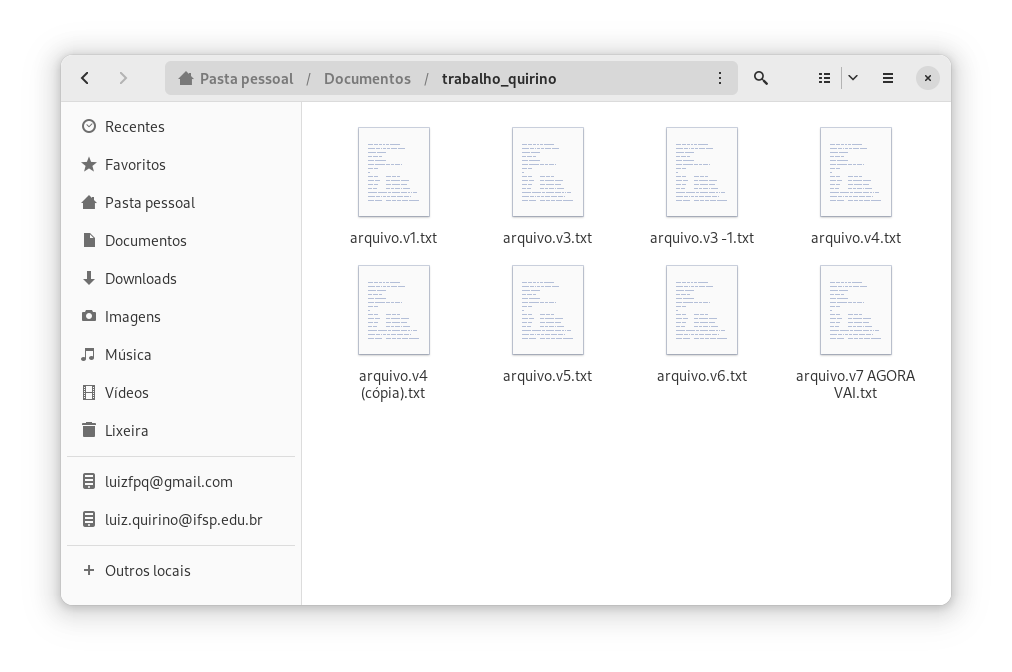
\includegraphics[width=1.0\textwidth]{assets/aula-tdsi-ifds-2023-05-24/Captura de tela de 2023-05-23 11-29-31.png}}
            \caption{Versionamento por arquivos}
        \end{figure}
\end{frame}

\begin{frame}[fragile]{Que tal isso aqui?}
      \begin{figure}[H]
            \centerline{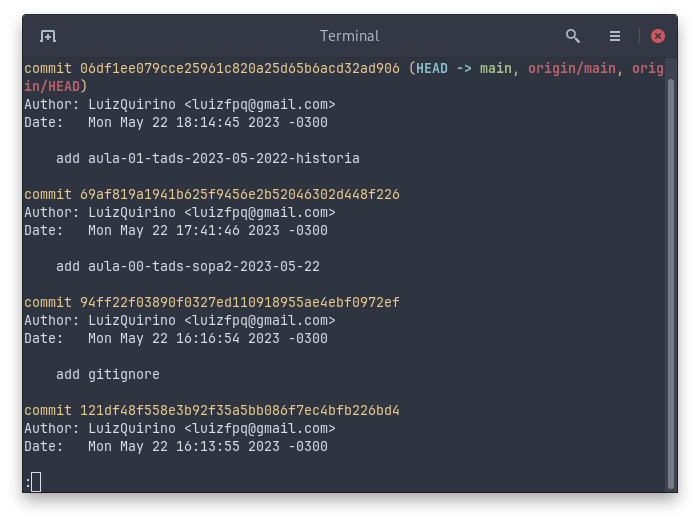
\includegraphics[width=0.9\textwidth]{assets/aula-tdsi-ifds-2023-05-24/Captura de tela de 2023-05-23 11-32-10.png}}
            \caption{git - terminal}
        \end{figure}
\end{frame}

\begin{frame}[fragile]{E essa belezinha aqui?}
      \begin{figure}[H]
            \centerline{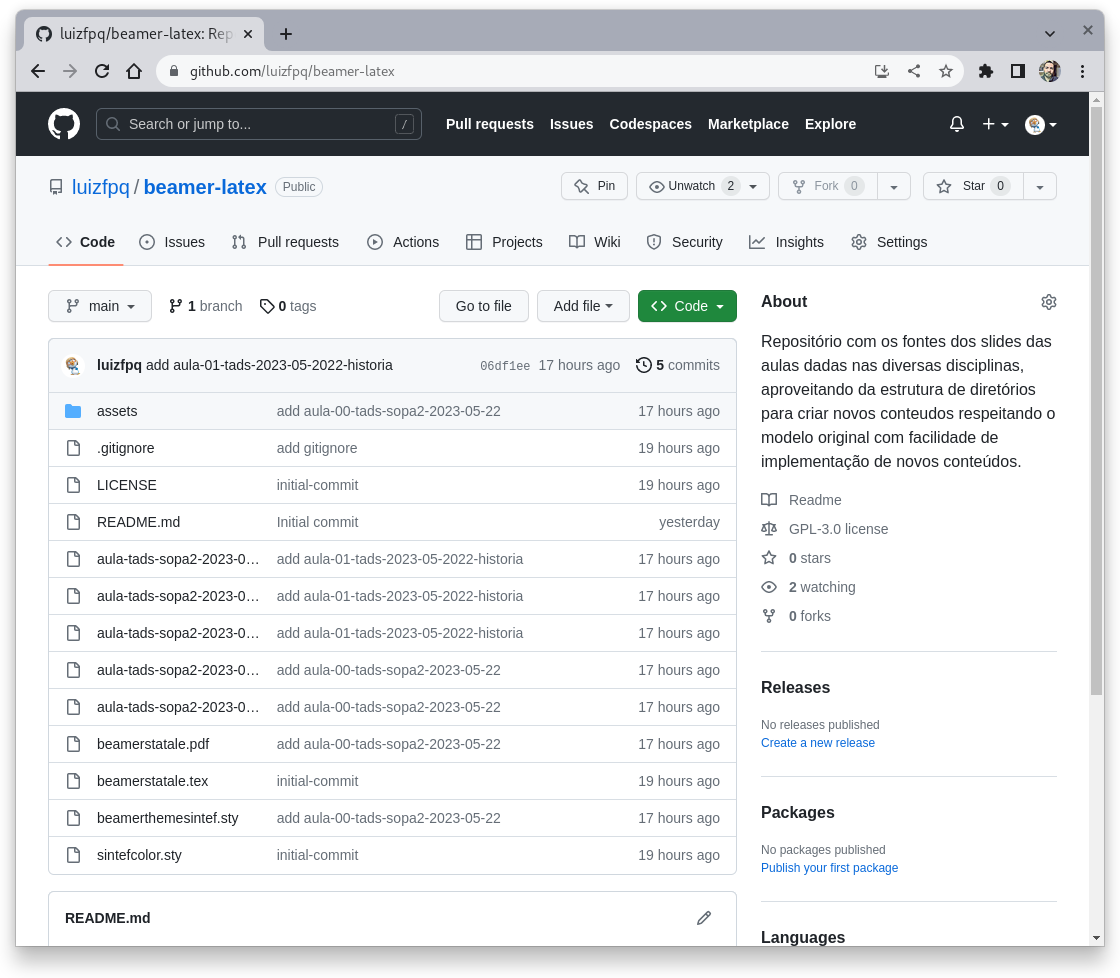
\includegraphics[width=0.9\textwidth]{assets/aula-tdsi-ifds-2023-05-24/Captura de tela de 2023-05-23 11-32-53.png}}
            \caption{repositório no github}
        \end{figure}
\end{frame}

\begin{frame}[fragile]{Vantagens}

      \begin{itemize}
            \item Controle do histórico
            \item Trabalho em equipe
            \item Marcação e resgate de versões estáveis
            \item Ramificação do projeto
      \end{itemize}
      \end{frame}

      




\begin{frame}[fragile]{Tipos de VCS}

      \begin{itemize}
            \item Sistemas de Controle de Versão Locais
            \item Sistemas de Controle de Versão Centralizados
            \item Sistemas de Controle de Versão Distribuidos
      \end{itemize}
      \end{frame}

\begin{frame}{Controle local}\justifying
      O método de controle de versão de muitas pessoas é copiar os arquivos para outro diretório (talvez um diretório com carimbo de tempo, se eles forem espertos). Esta abordagem é muito comum porque é muito simples, mas também é incrivelmente propensa a erros. É fácil esquecer em qual diretório você está e acidentalmente sobreescrever o arquivo errado ou copiar arquivos que não quer.
\end{frame}

\begin{frame}{Controle local} \justifying
      Uma das ferramentas VCS mais populares foi um sistema chamado RCS, que ainda é distribuído com muitos computadores hoje. Até mesmo o popular sistema operacional Mac OS X inclui o comando rcs quando você instala as Ferramentas de Desenvolvimento. RCS funciona mantendo conjuntos de alterações (ou seja, as diferenças entre os arquivos) em um formato especial no disco; ele pode, em seguida, re-criar como qualquer arquivo se parecia em qualquer ponto no tempo, adicionando-se todas as alterações.
\end{frame}

\begin{frame}[fragile]{Desenhando...}
      \begin{figure}[H]
            \centerline{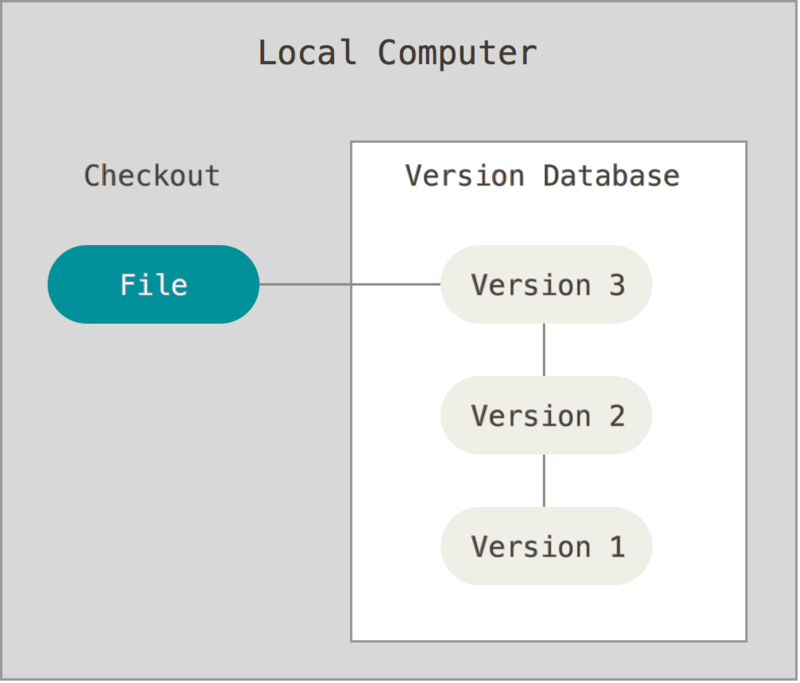
\includegraphics[width=0.5\textwidth]{assets/aula-tdsi-ifds-2023-05-24/controle-local.png}}
            \caption{Sistemas de controle local}
        \end{figure}
\end{frame}

\begin{frame}{Controle Centralizado (CVCS)} \justifying
      A próxima questão importante que as pessoas encontram é que elas precisam colaborar com desenvolvedores em outros sistemas. Para lidar com este problema, Sistemas Centralizados de Controle de Versão (CVCSs) foram desenvolvidos. Estes sistemas, tais como CVS, Subversion e Perforce, têm um único servidor que contém todos os arquivos de controle de versão, e um número de clientes que usam arquivos a partir desse lugar central. Por muitos anos, este tem sido o padrão para controle de versão.
\end{frame}

\begin{frame}{Controle Centralizado} \justifying
      Esta configuração oferece muitas vantagens, especialmente sobre VCSs locais. Por exemplo, todo mundo sabe, até certo ponto o que todo mundo no projeto está fazendo. Os administradores têm controle refinado sobre quem pode fazer o que; e é muito mais fácil de administrar um CVCS do que lidar com bancos de dados locais em cada cliente.
\end{frame}

\begin{frame}{Controle Centralizado} \justifying
      No entanto, esta configuração também tem algumas desvantagens graves. O mais óbvio é o ponto único de falha que o servidor centralizado representa. Se esse servidor der problema por uma hora, durante essa hora ninguém pode colaborar ou salvar as alterações de versão para o que quer que eles estejam trabalhando. Se o disco rígido do banco de dados central for corrompido, e backups apropriados não foram mantidos, você perde absolutamente tudo - toda a história do projeto, exceto imagens pontuais que desenvolvedores possam ter em suas máquinas locais. Sistemas VCS locais sofrem com esse mesmo problema - sempre que você tenha toda a história do projeto em um único lugar, há o risco de perder tudo.
\end{frame}



\begin{frame}[fragile]{Desenhando...}
      \begin{figure}[H]
            \centerline{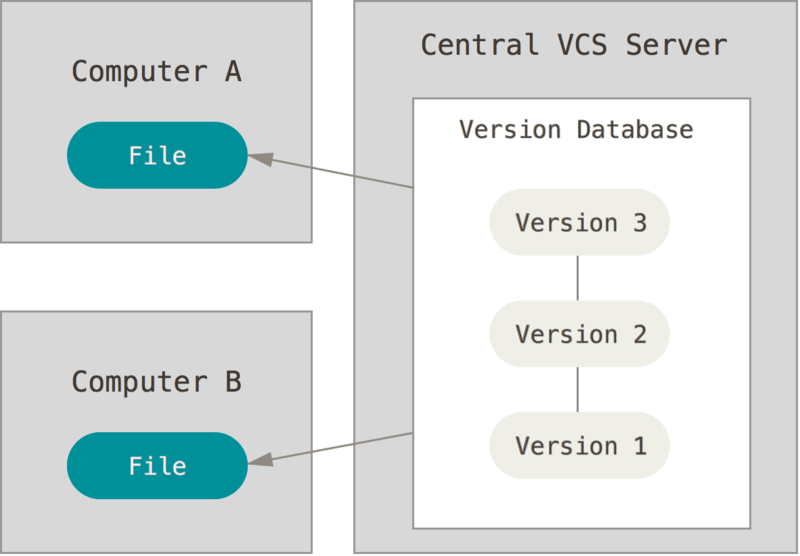
\includegraphics[width=0.5\textwidth]{assets/aula-tdsi-ifds-2023-05-24/controle-centralizado.png}}
            \caption{Sistemas de controle Centralizado}
        \end{figure}
\end{frame}

\begin{frame}{Controle distribuído (DVCS)} \justifying
      E foi assim que Sistemas Distribuídos de Controle de Versão (DVCS) entram em cena. Em um DVCS (como Git, Mercurial, Bazaar ou Darcs), clientes não somente usam o estado mais recente dos arquivos: eles duplicam localmente o repositório completo. Assim, se qualquer servidor morrer, e esses sistemas estiverem colaborando por meio dele, qualquer um dos repositórios de clientes podem ser copiado de volta para o servidor para restaurá-lo. Cada clone é de fato um backup completo de todos os dados.
\end{frame}

\begin{frame}{Controle distribuído} \justifying
      Além disso, muitos desses sistemas trabalham muito bem com vários repositórios remotos, tal que você possa colaborar em diferentes grupos de pessoas de maneiras diferentes ao mesmo tempo dentro do mesmo projeto. Isso permite que você configure vários tipos de fluxos de trabalho que não são possíveis em sistemas centralizados, como modelos hierárquicos.
\end{frame}


\begin{frame}[fragile]{Desenhando...}
      \begin{figure}[H]
            \centerline{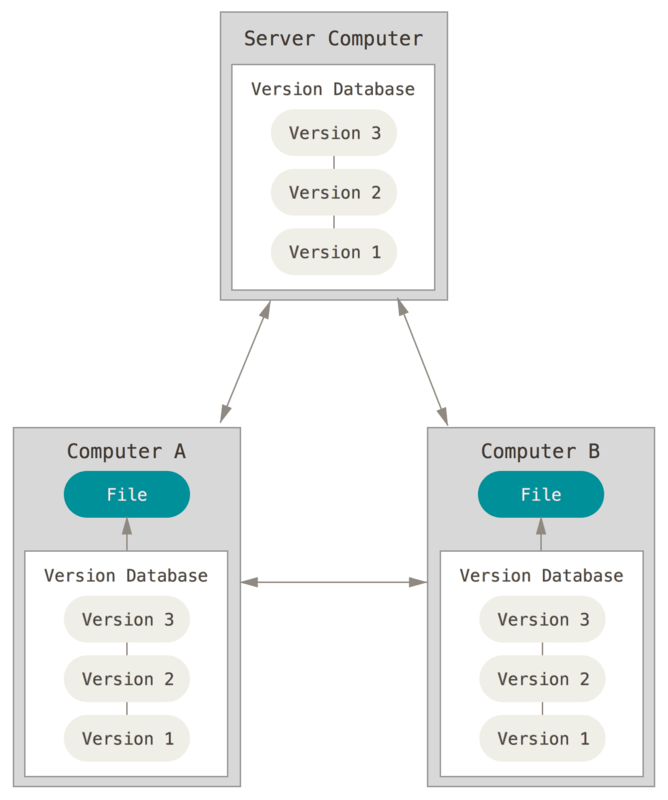
\includegraphics[width=0.35\textwidth]{assets/aula-tdsi-ifds-2023-05-24/controle-distribuido.png}}
            \caption{Sistemas de controle distribuido}
        \end{figure}
\end{frame}

\begin{frame}[fragile]{Exemplos de sistemas de controle de versão}

      \begin{itemize}
            \item CVS - Livre
            \item \textbf{Git} - Livre
            \item SVN - Livre
            \item SourceSafe - Microsoft
            \item ClearCase - IBM
            
      \end{itemize}
      \end{frame}

\section{Com o que trabalharemos?}
\begin{frame}{Uma breve história do Git} \justifying
      Como muitas coisas na vida, o Git começou com um pouco de destruição criativa e uma ardente controvérsia.
      \\...
      \\O núcleo (kernel) do Linux é um projeto de código aberto com um escopo bastante grande. A maior parte da vida da manutenção do núcleo o Linux (1991-2002), as mudanças no código eram compartilhadas como correções e arquivos. Em 2002, o projeto do núcleo do Linux começou usar uma DVCS proprietária chamada BitKeeper.
\end{frame}

\begin{frame}{Uma breve história do Git} \justifying
      Em 2005, a relação entre a comunidade que desenvolveu o núcleo do Linux e a empresa que desenvolveu BitKeeper quebrou em pedaços, e a ferramenta passou a ser paga. Isto alertou a comunidade que desenvolvia o Linux (e especialmente Linus Torvalds, o criador do Linux) a desenvolver a sua própria ferramenta baseada em lições aprendidas ao usar o BitKeeper. 
\end{frame}

\begin{frame}{Uma breve história do Git} \justifying
      Algumas metas do novo sistema era os seguintes:
      \begin{itemize}
            \item Velocidade
            \item Projeto simples
            \item Forte suporte para desenvolvimento não-linear (milhares de ramos paralelos)
            \item Completamente distribuído
            \item Capaz de lidar com projetos grandes como o núcleo o Linux com eficiência (velocidade e tamanho dos dados)
      \end{itemize}
\end{frame}

\begin{frame}{Uma breve história do Git} \justifying
      Desde seu nascimento em 2005, Git evoluiu e amadureceu para ser fácil de usar e ainda reter essas qualidades iniciais. Ele é incrivelmente rápido, é muito eficiente com projetos grandes, e ele tem um incrível sistema de ramos para desenvolvimento não linear.
\end{frame}


\subsection{Trabalhando com a nossa ferramenta}

\begin{frame}{Maneiras de trabalhar}\justifying
      Existem várias formas diferentes de usar o Git. Existem as ferramentas originais de linha de comando, e existem várias interfaces gráficas de usuário (GUI - Graphical User Interface) com opções variadas.\\ Nós \textbf{inicialmente} usaremos o Git na linha de comando. 
      A linha de comando é o único lugar onde você pode rodar todos os comandos do Git - 
      a maioria das GUI implementa somente um subconjunto das funcionalidades do Git. 
      \\Se você sabe como usar o Git na linha de comando, você provavelmente descobrirá como 
      rodar versões GUI, enquanto o oposto não é necessariamente verdade. 
      Além disso, enquanto a sua escolha da interface gráfica é uma questão de gosto pessoal, todos os usuário terão as ferramentas de linha de comando instaladas e disponíveis.
\end{frame}

\section{Atividade}

\begin{frame}{Criar nosso primeiro repositório}
      \begin{itemize}
            \item Testar o uso do nosso primeiro repositório local.
            \item Testar o uso de um repositório Git
            \item Debater sobre as diferenças e possibiliades
      \end{itemize}
\end{frame}

\backmatter
\end{document}
